\documentclass[11pt]{article}

% --- Page layout ---
\usepackage[a4paper,margin=2cm]{geometry}

% --- Typography and section formatting ---
\usepackage{titlesec}
\titleformat{\section}{\normalfont\Large\bfseries}{}{0pt}{}
\titleformat{\subsection}{\normalfont\large\bfseries}{}{0pt}{}
\usepackage{parskip}

% --- Figures and tables ---
\usepackage{graphicx}
\usepackage{float}
\usepackage{booktabs}
\usepackage{caption}
\usepackage{subcaption}
\captionsetup[figure]{justification=centering}
\usepackage{url}
\usepackage{booktabs}
\usepackage{array}
\newcolumntype{M}[1]{>{\centering\arraybackslash}m{#1}}
\usepackage{amsmath}

% --- Document starts here ---
\begin{document}
	
	\begin{center}
		\LARGE\textbf{Bayesian Spatial Risk Modelling of Suicide Mortality in South Korea Using the ICAR Model}
	\end{center}
	
	\section*{Introduction}
	
	South Korea consistently reports one of the highest suicide rates among developed nations, with 24 to 28 deaths per 100,000 people in recent years—nearly twice the OECD average of 11 (Kim, 2024). Although rates declined modestly in the mid-2010s following national prevention efforts, they have since resurged, reaching 28.3 per 100,000 in 2024—the highest level in over a decade (YNA, 2025). This persistent trend positions South Korea as a global outlier and underscores the urgent need to investigate its underlying risk factors. A large body of research shows that suicide rates are shaped by a mix of socioeconomic, demographic, cultural, and psychological factors. Classic theories dating back to Durkheim (1951) emphasise the protective role of social integration, while economic hardship and mental illness remain key drivers. In South Korea, national crises such as the late 1990s Asian financial crash have been linked to suicide spikes, primarily through rising unemployment and social dislocation (Chang, 2009).
	
	Among the many determinants examined, social isolation have been identified as a major risk factor. Individuals living alone or lacking family support are more vulnerable due to loneliness and reduced integration. In South Korea, areas with more single-person households or divorced residents tend to have higher suicide rates (Jang, 2022), reflecting the link between weaker social ties and suicide risk. Psychological stress is another significant factor. South Korea reports high levels of perceived stress, which is associated with depression and suicide ideation (Oh, 2020). The indicator "stress awareness"—the proportion of people experiencing significant stress—has been linked to higher suicide rates at the regional level (Jang, 2022). Unemployment is a well-documented driver. Job loss can trigger financial strain, identity loss, and psychological distress. Park and Lester (2006) identified unemployment as a key contributor to South Korea's suicide rate, particularly where social safety nets are weak. Lastly, unmet medical needs reflect gaps in healthcare access, including mental health services. Though 90\% of people who die by suicide have a diagnosable condition, only about 15\% ever receive treatment. Kim (2022) finds that regions with higher unmet medical needs tend to experience higher suicide mortality.
	
	Given the spatially patterned nature of suicide, advanced statistical methods are needed to separate risk factors from geographic influences. We use a Bayesian Intrinsic Conditional Auto-Regressive (ICAR) model, which incorporates information from adjacent regions to produce more stable small-area risk estimates. Our analysis includes four key covariates discussed above, alongside spatial random effects to assess their contribution to geographic variation. This modelling framework accounts for unobserved spatial influences and estimates exceedance probabilites to identify municipalities where suicide risk surpasses a defined threshold. Our key outputs will provide localised insights into suicide risk and guide targeted public health interventions and efficient resource allocation across South Korea.

	\section*{1. Data and Methods}
	
	\subsection*{1.1 Study Area and Spatial Units}
	
	The study area comprises all local government units in South Korea, including metropolitan cities, special administrative regions, and provinces, aggregated to the municipality level for analytical consistency. Administrative boundaries were derived from 2022 shapefiles and subsequently harmonised with statistical datasets from various sources.
	
	\subsection*{1.2 Target and Predictor Variables}
	
	The primary outcome variable is the number of suicide casualties in 2022, computed using suicide rates (per 100,000 population) and registered population figures. Four predictor variables were selected based on literature and data availability:
	
	Define variables here.
	
	\begin{table}[H]
		\centering
		\caption{Summary of Datasets Used in the Analysis}
		\renewcommand{\arraystretch}{1.4}
		\resizebox{\textwidth}{!}{%
			\begin{tabular}{M{4.5cm} M{4.5cm} M{3.5cm} M{5cm} M{1.2cm}}
				\toprule
				\textbf{Variable} & \textbf{Dataset} & \textbf{Usage} & \textbf{Source} & \textbf{Year} \\
				\midrule
				\textbf{Suicide Rate} & Cause of Death Statistics & Target variable & Statistics Korea (Population Trends Division) & 2022 \\
				\textbf{Single-Person Household Ratio} & Population and Housing Census & Predictor variable & Statistics Korea (Population and Housing Census Division) & 2022 \\
				\textbf{Stress Awareness Rate} & Community Health Survey & Predictor variable & Korea Disease Control and Prevention Agency (KDCA) & 2022 \\
				\textbf{Unemployment Rate} & Local Employment Statistics & Predictor variable & Statistics Korea (Employment Statistics Division) & 2022 \\
				\textbf{Unmet Medical Needs Rate} & Community Health Survey & Predictor variable & Korea Disease Control and Prevention Agency (KDCA) & 2022 \\
				\textbf{Estimated Population} & Future Population Projections & Standardisation / Denominator & Statistics Korea (Regional Statistics Planning Division) & 2022 \\
				\textbf{Municipality Boundaries} & Municipality Shapefiles & Spatial analysis & GIS Developer & 2022 \\
				\textbf{Province Boundaries} & Province Shapefiles & Mapping / Labelling & GIS Developer & 2022 \\
				\bottomrule
			\end{tabular}
		}
		\label{tab:datasets}
	\end{table}
	
	
	All covariates reflect conditions in 2022. Municipality-level datasets were retrieved from national public databases, then cleaned and merged based on administrative codes and names.
	
	\begin{figure}[H]
		\centering
		\caption{Suicide Rates Across South Korean Municipalities}
		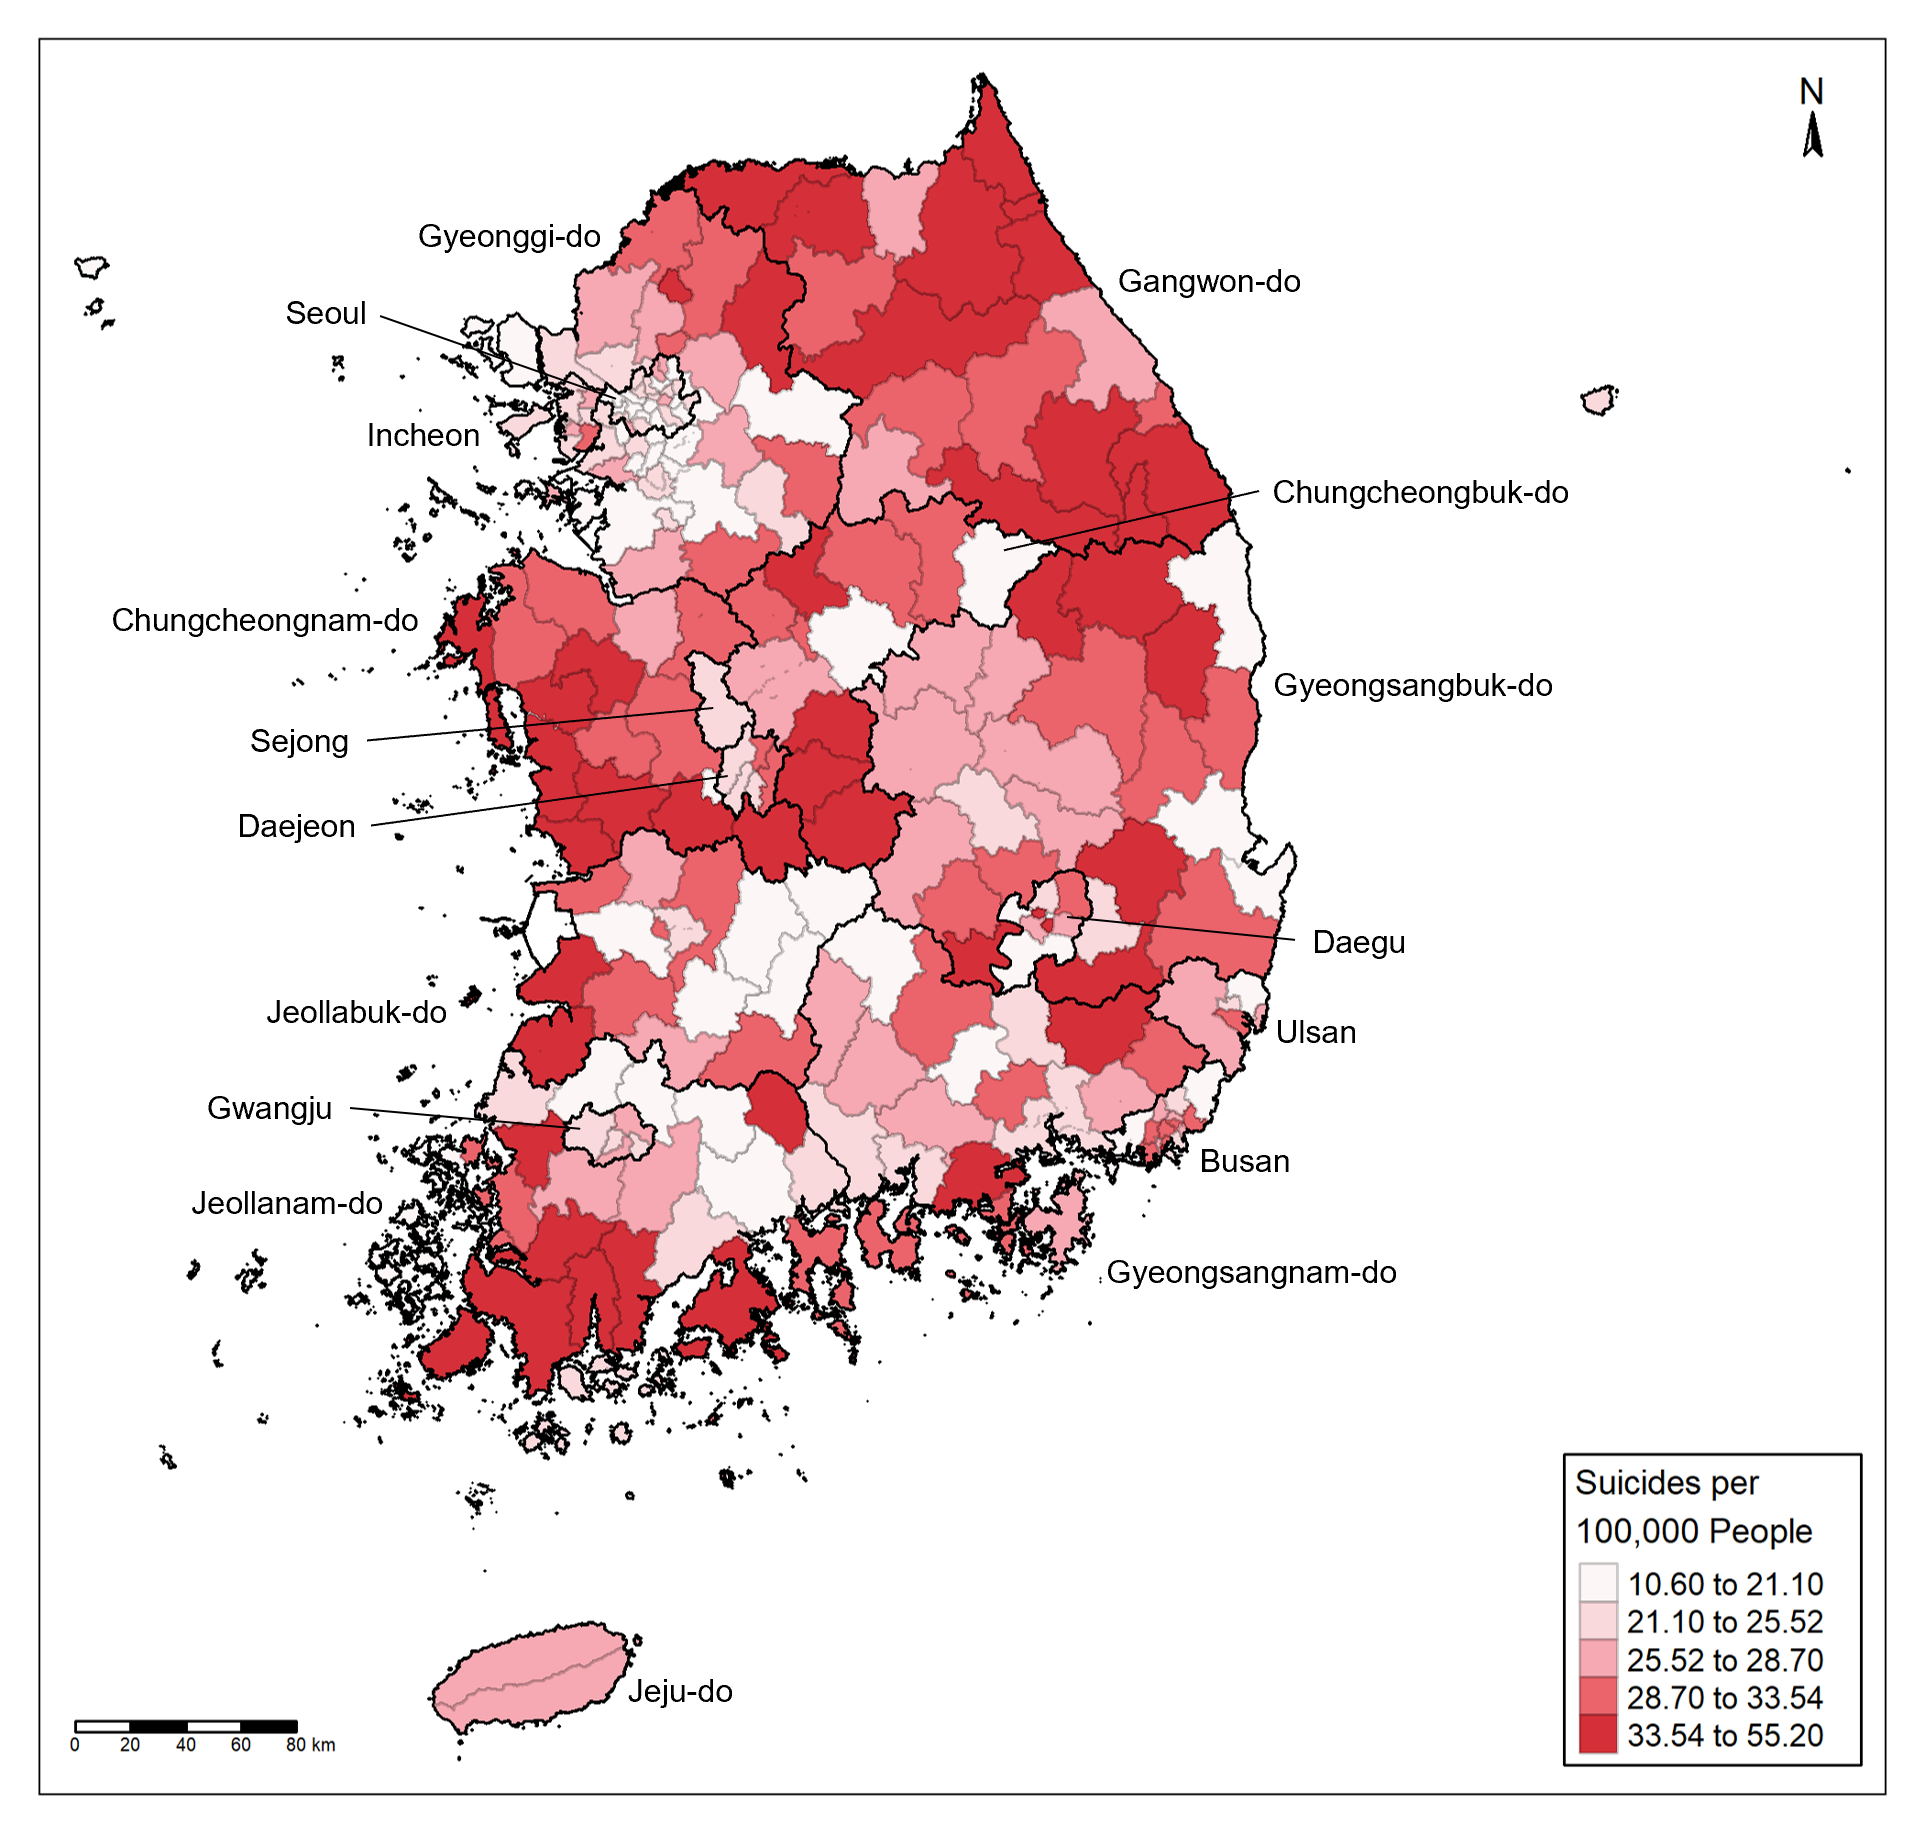
\includegraphics[width=1\textwidth]{assets/suicide_map/suicide_map_2022_annotated.png}
	\end{figure}


	\subsection*{1.3 Model Specification}
	
	We applied a Bayesian Poisson model incorporating an ICAR prior to account for spatial autocorrelation among neighbouring municipalities. The model estimates relative risk (RR) of suicide for each area, using the expected number of cases (based on population) as an offset:

	\begin{equation}
		Y_i \sim \text{Poisson}(\lambda_i), \quad 
		\log(\lambda_i) = \log(E_i) + \alpha + \mathbf{X}_i \boldsymbol{\beta} + \sigma \cdot \phi_i\footnote{In the full model, we include both structured and unstructured random effects: 
			$\log(\lambda_i) = \log(E_i) + \alpha + \mathbf{X}_i \boldsymbol{\beta} + \sigma \cdot \left( \sqrt{1 - \rho} \, \theta_i + \sqrt{\rho} \, \phi_i \right)$, where $\theta_i \sim \mathcal{N}(0,1)$ captures unstructured heterogeneity and $\phi_i$ follows an ICAR prior for spatial structure.}
	\end{equation}
	
	
%	Where $Y_i$ is the observed count, $E_i$ the expected count, $\alpha$ the intercept, $\mathbf{X}_i$ the matrix of covariates, $\boldsymbol{\beta}$ their respective coefficients, $\phi_i$ the spatial random effect (structured), and $\sigma$ the scaling term.
%	
%	We employed a hybrid random effect combining spatially structured (ICAR) and unstructured (Gaussian) components. Priors were defined as follows:
%	\begin{itemize}
%		\item $\alpha \sim \mathcal{N}(0, 1)$
%		\item $\boldsymbol{\beta} \sim \mathcal{N}(0, 1)$
%		\item $\theta_i \sim \mathcal{N}(0,1)$
%		\item $\phi \sim \text{ICAR}$
%		\item $\rho \sim \text{Beta}(0.5, 0.5)$
%	\end{itemize}
%	
%	Model fitting was performed in \textit{Stan} via the \textit{rstan} interface, using 6 chains, 20,000 iterations, and a burn-in of 10,000.
%	
	\section*{2. Results and Discussion}
	
	\subsection*{2.1 Global Parameter Estimates}
	
	The model converged successfully with all $\hat{R}$ values below 1.05 and high effective sample sizes. Table 1 summarises posterior estimates:
	
	\begin{table}[H]
		\centering
		\caption{Posterior Estimates of Global Parameters}
		\renewcommand{\arraystretch}{1.3}
		\begin{tabular}{ccccccc}
			\hline
			\textbf{Parameter} & \textbf{Mean} & \textbf{2.5\% CrI } & \textbf{97.5\% CrI } & \boldmath{$n_\text{eff}$} & \boldmath{$\hat{R}$} \\
			\hline
			$\alpha$   & $-0.1956$ & $-0.4548$ & $0.0685$ & $25689.1$ & $1.0005$ \\
			$\beta_1$  & $0.0120$ & $0.0067$  & $0.0174$ & $27152.2$ & $1.0003$ \\
			$\beta_2$  & $-0.0052$ & $-0.0139$ & $0.0035$ & $26780.3$ & $1.0001$ \\
			$\beta_3$  & $-0.0385$ & $-0.0706$ & $-0.0065$ & $9776.5$ & $1.0007$ \\
			$\beta_4$  & $0.0089$ & $-0.0014$ & $0.0190$ & $28092.1$ & $1.0001$ \\
			$\sigma$   & $0.2118$ & $0.1611$  & $0.2685$ & $7507.3$ & $1.0006$ \\
			\hline
		\end{tabular}
		\vspace{0.5em}
		\begin{minipage}{0.95\textwidth}
			\footnotesize
			\textit{Note.} CrI = Credible Interval; $n_\text{eff}$ indicates the effective sample size from the posterior. $\hat{R}$ denotes the Gelman-Rubin convergence diagnostic, with values close to 1.00 indicating good convergence.
		\end{minipage}
		\label{tab:icar_results}
	\end{table}
%	
%	Unemployment shows the strongest association with suicide risk, with a 4\% decrease in relative risk per unit increase. Conversely, single-person household and unmet medical needs each correspond to a 1\% increase in risk. Stress awareness shows a small, borderline significant negative association.
%	
%	\subsection*{2.2 Spatial Distribution of Relative Risk}
%	
%	\begin{figure}[H]
%		\centering
%		\includegraphics[width=0.8\textwidth]{assets/rr_map.png}
%		\caption{Relative Risk of Suicide across South Korea}
%	\end{figure}
%	
%	Figure 1 displays the relative risk estimates per municipality. Most areas exhibit RRs between 0.95 and 1.10, indicating modest spatial variability. However, some peripheral provinces and rural municipalities show elevated risks, while Seoul and its metropolitan surroundings tend to have reduced risk.
%	
%	\subsection*{2.3 Statistical Significance of RR}
%	
%	\begin{figure}[H]
%		\centering
%		\includegraphics[width=0.8\textwidth]{assets/significance_map.png}
%		\caption{Significance of Relative Risk Estimates}
%	\end{figure}
%	
%	Figure 2 shows areas with statistically significant deviations from the national average risk. Red areas represent significantly elevated risk ($RR > 1$), while blue areas indicate significantly reduced risk. The vast majority are non-significant (white), yet spatial clustering is evident in both high- and low-risk zones.
%	
%	\subsection*{2.4 Exceedance Probabilities}
%	
%	\begin{figure}[H]
%		\centering
%		\includegraphics[width=0.8\textwidth]{assets/exceedance_prob_map.png}
%		\caption{Exceedance Probabilities ($P(RR > 1)$)}
%	\end{figure}
%	
%	Exceedance probabilities (Figure 3) provide an intuitive measure of uncertainty. Regions in the southeast and some interior provinces exhibit probabilities exceeding 0.90, strongly suggesting elevated suicide risk. In contrast, capital regions show probabilities below 0.10.
%	
%	\subsection*{2.5 Policy Implications and Interpretation}
%	
%	Spatial analysis reveals a pronounced urban-rural divide. Rural areas, especially those with high proportions of single-person households and unmet health needs, face elevated risks. Policymakers should prioritise these areas for mental health outreach, economic support, and healthcare infrastructure.
%	
%	Moreover, the inverse relationship between unemployment and suicide risk may reflect complex socio-economic mechanisms, including the effects of underemployment or economic pressures in high-cost urban areas. This finding warrants deeper exploration.
%	
%	\section*{Conclusion}
%	
%	This study highlights the value of spatial Bayesian modelling in understanding suicide risk across South Korea. By applying an ICAR model to municipal data, we identified significant geographic disparities and contextualised them via socio-economic indicators. The approach enables robust risk estimation while accounting for spatial dependencies and uncertainty.
%	
%	The findings underline the importance of targeted public health strategies that go beyond national averages. Regional policies, especially in rural and underserved areas, must consider unique social determinants of suicide and leverage geospatial evidence for efficient intervention planning.
%	
%	\section*{References}
%	
%	\begin{flushleft}
%		\begin{thebibliography}{9}
%			\bibitem{WHO2023}
%			World Health Organization. (2023). \textit{Suicide Worldwide in 2022: Global Health Estimates}. Geneva: WHO.
%			
%			\bibitem{Rue2005}
%			Rue, H., Martino, S., & Chopin, N. (2009). \textit{Approximate Bayesian inference for latent Gaussian models using integrated nested Laplace approximations (INLA)}. Journal of the Royal Statistical Society, Series B, 71(2), 319--392.
%			
%			\bibitem{Lee2011}
%			Lee, D. (2011). \textit{A comparison of conditional autoregressive models used in Bayesian disease mapping}. Spatial and Spatio-temporal Epidemiology, 2(2), 79--89.
%			
%			\bibitem{Zhu2006}
%			Zhu, L., Gorman, D. M., & Horel, S. (2006). \textit{Hierarchical Bayesian spatial models for alcohol availability, drug "hot spots," and violent crime}. International Journal of Health Geographics, 5(1), 54.
%			
%			\bibitem{StatisticsKorea2022}
%			Statistics Korea. (2023). \textit{Population and Health Indicators by Municipality}. Daejeon: KOSIS.
%		\end{thebibliography}
%	\end{flushleft}

%Kim, E. and Kim, S. (2024). Spatially clustered patterns of suicide mortality rates in South Korea: a geographically weighted regression analysis. BMC Public Health, 24(1). doi:https://doi.org/10.1186/s12889-024-19899-4.
	
\end{document}

